\documentclass[fleqn]{hermans-hw}

\usepackage{url}
\usepackage{graphicx}
\usepackage{amsmath}
\usepackage[linewidth=1pt, leftmargin=0,rightmargin=0, innertopmargin = \topskip,splittopskip=\topskip, innerleftmargin=2,innerrightmargin=10]{mdframed}
\topmargin -1.5cm        % read Lamport p.163
\oddsidemargin -0.04cm   % read Lamport p.163
\evensidemargin -0.04cm  % same as oddsidemargin but for left-hand pages
\textwidth 16.59cm
\textheight 21.94cm
\parskip 7.2pt           % sets spacing between paragraphs

\newcommand{\BP}{\mathbf{P}}

\title{HW9: Hidden Markov Models}
\class{CS 4300: Artificial Intelligence}
\institute{University of Utah}
\author{William Frank, u1067292}
% IF YOU'RE USING THIS .TEX FILE AS A TEMPLATE, PLEASE REPLACE
% The author WITH YOUR NAME AND UID.
% Replace the due date with anyone you worked with i.e. "Worked with: John McCarthy, Watson, & Hal-9000"
\begin{document}
\maketitle
\section{Stationary Distributions of Markov Chains}

Alice decides that she wants to keep re-taking AI every semester for
the rest of eternity (she \emph{really} likes AI).  We're interested
in modeling whether she passes the class or not as a Markov chain.
Suppose that in semester $t$ she passes the class; then in semester
$t+1$ she passes the class with probability $0.8$ (maybe she gets
bored and forgets to pay attention).  On the other hand, if she
doesn't pass in semester $t$ then she'll pass with probability $0.4$.

\begin{enumerate}
\item Suppose that in semester $t=0$ Alice passes the class with
  probability $0.5$.  Compute the probability that she passes in
  semester $t=1$ and semester $t=2$.
  
	$P(p_{t=1}, p_{t=0}) = 0.4$
  
	$P(p_{t=1}, f_{t=0}) = 0.2$
	
	$P(p_{t=1}) = 0.6$
	
	\bigskip
  
	$P(p_{t=2}, p_{t=1}, p_{t=0}) = 0.32$

	$P(p_{t=2}, p_{t=1}, f_{t=0}) = 0.16$
	
	$P(p_{t=2}, f_{t=1}, p_{t=0}) = 0.04$
	
	$P(p_{t=2}, f_{t=1}, f_{t=0}) = 0.12$
	
	$P(p_{t=2}) = 0.64$
	
\item Compute the stationary distribution of this chain.  (Hint: the
  easiest way to do this is to start with some ``guess'' -- say 50/50
  -- and then keep simulating the chain for a while until it seems to
  settle down.  Once you think you've got a guess at what the
  stationary distribution might be, try transitioning from there to
  see if you get back to the stationary distribution.)  (Not as
  helpful hint: if you like linear algebra, you can directly compute
  the stationary distribution from the transition matrix using an
  eigenvalue decomposition: take a look at Wikipedia for how!)
  
	$\BP = 
	\begin{pmatrix}
	0.8 & 0.2 \\
	0.4 & 0.6 \\
	\end{pmatrix}$
	
	$det(\BP - \lambda\mathbf{I}) = 0 \rightarrow \lambda = 0.4, 1$
	
	Eigenvectors = $\begin{pmatrix} -0.5 \\ 1 \\ \end{pmatrix}$ and $\begin{pmatrix} 1 \\ 1 \\ \end{pmatrix}$
	
	Therefore the stationary distribution is $\begin{pmatrix} 0.5 \\ 0.5 \\ \end{pmatrix}$
  
\end{enumerate}
\vspace{-0.5cm}
\section{Alice and the Crazy Coke Machine}
\vspace{-0.5cm}
Alice is up late studying for her algorithms final exam and needs to
stay hydrated (and caffeinated!).  Unfortunately, Clarence was the one
who bought the soda machine in the lab.  He went for the cheapest
model.  All you can do with this soda machine is put money in and hope
it gives you the type of drink you want.  It carries three types of
soda: Coke (C), Diet Coke (D) and Sprite (S).

Alice has been monitoring the soda machine for a while and has figured
out that it behaves as an HMM.  It has two internal states (call them
A and B).  When asked for a soda from state A, it gives a coke with
probability 1/2, and a diet coke and a sprite each with probability
1/4.  On the other hand, when asked for a soda in state B, it gives a
diet coke with probability 1/2, a sprite with probability 1/3 and a
coke with probability 1/6.  Furthermore, it transitions from state A
to A with probability 4/5 and from state B to B with probability 3/5.

The machine formally works as follows.  It is in some state $s$.
Someone puts in money and it dispenses a soda according to the
probability rules set out above, being in state $s$.  It then
(randomly) transitions to a new state $s'$ according to the transition
probabilities above.

\begin{enumerate}
\item Draw a state space lattice for this soda machine (as on the slides from HMM) for three time steps.

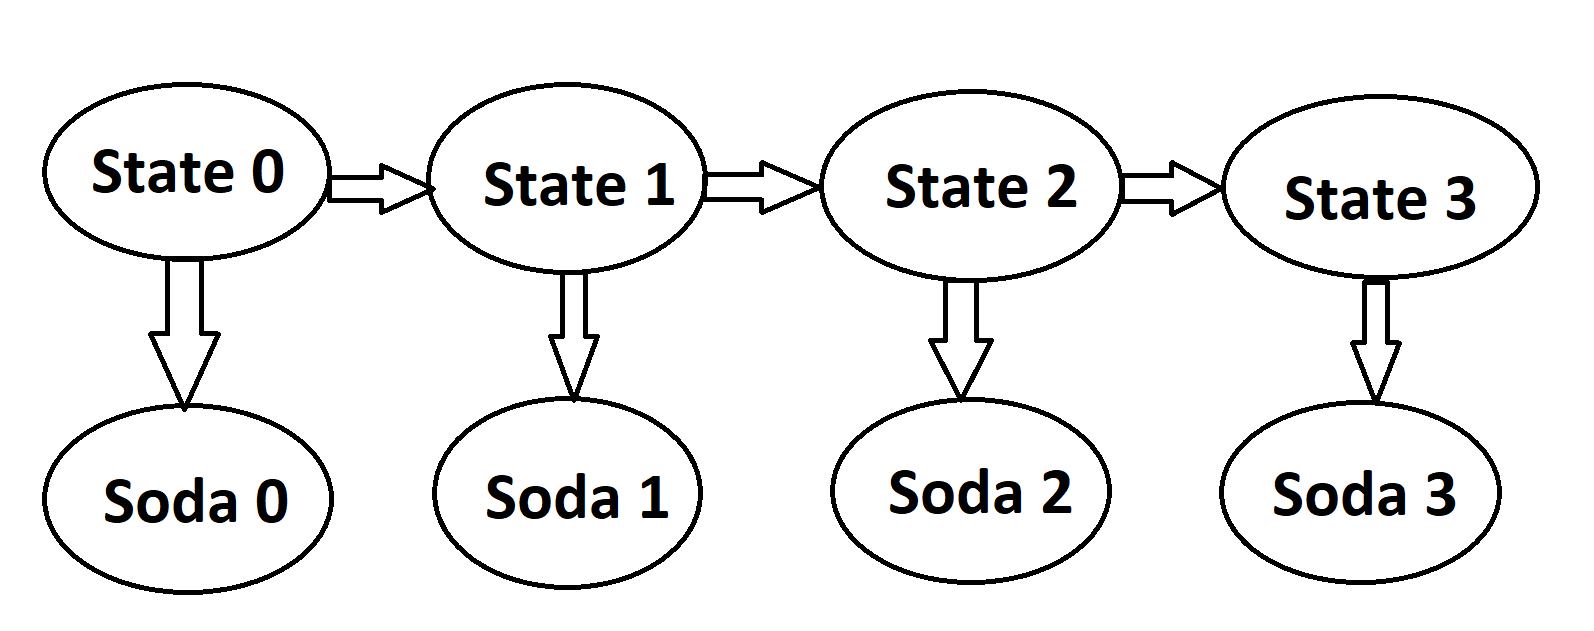
\includegraphics[scale=0.8]{state-lattice.png}

\item Suppose that Alice doesn't know what state the machine is in
  currently (specifically, she believes it's equally likely to be in
  either state), but puts money in and gets a Sprite out.  What is the
  probability distribution over states that it was in when Alice put
  her money in?  What is the probability distribution over states that
  it is in now?
  
  Initially:
  
  P(A $|$ S) = P(A) P(S $|$ A) = (.5)(.25) = .125 $\rightarrow$ 3/7
  
  P(B $|$ S) = P(B) P(S $|$ B) = (.5)(.333) = .167 $\rightarrow$ 4/7
  
  After:
  
  P(A) = P(A) P(A $|$ A) + P(B) P(A $|$ B) = (.5)(.8) + (.5)(.4) = 0.6
  
  P(B) = P(B) P(B $|$ B) + P(A) P(B $|$ A) = (.5)(.6) + (.5)(.2) = 0.4

\item Suppose Alice comes back the next day (so again she doesn't know
  what state the machine is in) and really wants a diet coke.
  Unfortunately, the machine isn't being particularly nice to her and
  it produces the following series of emissions upon taking money from
  Alice: C S S D.  What is the most likely sequence of states the
  machine went through in this process?
  
	Soda 1:
	
	$m_1(A) = P(C|A) P(A) = (.5)(.5) = .25$

	$m_1(B) = P(C|B) P(B) = (.167)(.5) = .083$
	
	\bigbreak
	
	Soda 2:
	
	$m_2(A) = P(S|A) max_{x_1}
	\begin{cases} 
	P(A|B) m_1(B) \\
	P(A|A) m_1(A) \\
	\end{cases}
	 =
	(.25) max_{x_1} \begin{cases} 
	(.4) (.083) \\
	(.8) (.25) \\
	\end{cases} = (.25)(.8)(.25) = .05
	$
	
	$m_2(B) = P(S|B) max_{x_1}
	\begin{cases} 
	P(B|B) m_1(B) \\
	P(B|A) m_1(A) \\
	\end{cases}
	=
	(.333) max_{x_1} \begin{cases} 
	(.6) (.083) \\
	(.2) (.25) \\
	\end{cases} = (.333)(.6)(.083) = .017
	$

	\bigbreak
	
	Soda 3:
	
	$m_3(A) = P(S|A) max_{x_2}
	\begin{cases} 
	P(A|B) m_2(B) \\
	P(A|A) m_2(A) \\
	\end{cases}
	=
	(.25) max_{x_2} \begin{cases} 
	(.4) (.017) \\
	(.8) (.05) \\
	\end{cases} = (.25)(.8)(.05) = .01
	$
	
	$m_3(B) = P(S|B) max_{x_2}
	\begin{cases} 
	P(B|B) m_2(B) \\
	P(B|A) m_2(A) \\
	\end{cases}
	=
	(.333) max_{x_2} \begin{cases} 
	(.6) (.017) \\
	(.2) (.05) \\
	\end{cases} = (.333)(.6)(.017) = .0034
	$
	
	\bigbreak
	
	Soda 4:
	
	$m_4(A) = P(D|A) max_{x_3}
	\begin{cases} 
	P(A|B) m_3(B) \\
	P(A|A) m_3(A) \\
	\end{cases}
	=
	(.25) max_{x_3} \begin{cases} 
	(.4) (.0034) \\
	(.8) (.01) \\
	\end{cases} = (.25)(.8)(.01) = .002
	$
	
	$m_3(B) = P(D|B) max_{x_3}
	\begin{cases} 
	P(B|B) m_3(B) \\
	P(B|A) m_3(A) \\
	\end{cases}
	=
	(.5) max_{x_3} \begin{cases} 
	(.6) (.0034) \\
	(.2) (.01) \\
	\end{cases} = (.5)(.6)(.0034) = .00102
	$
	
	\bigbreak
	
	Therefore, the most likely sequence of states is: \textit{A, A, A, A}
	  
\end{enumerate}
\end{document}

%%% Local Variables:
%%% mode: latex
%%% TeX-master: t
%%% End:
